\documentclass[11pt,a4paper]{article}
\usepackage[utf8]{inputenc}
\usepackage[english]{babel}	%Idioma
\usepackage{amsmath}
\usepackage{amsfonts}
\usepackage{amssymb}
\usepackage{graphicx} 	%Añadir imágenes
\usepackage{geometry}	%Ajustar márgenes
\usepackage[export]{adjustbox}[2011/08/13]
\usepackage{float}
\restylefloat{table}
\usepackage{booktabs}
\usepackage[hidelinks]{hyperref} %Con opción para eliminar los bordes rojos
\usepackage{titling}
%\usepackage{minted}
\usepackage{multirow}
\usepackage{caption}
\usepackage{multicol}
\usepackage[shortlabels]{enumitem}
\usepackage{array}
\usepackage{xcolor}
\selectlanguage{english}

%Para dibujar autómatas
\usepackage{tikz}
\usetikzlibrary{automata,positioning,arrows}

%Opciones de encabezado y pie de página:
\usepackage{fancyhdr}
\pagestyle{fancy}
\lhead{Nazaret Román Guerrero}
\rhead{Modelos de Computación}
\lfoot{Grado en Ingeniería Informática}
\cfoot{}
\rfoot{\thepage}
\renewcommand{\headrulewidth}{0.4pt}
\renewcommand{\footrulewidth}{0.4pt}

%Opciones de fuente:
\usepackage[utf8]{inputenc}
\usepackage{sourcecodepro}
\usepackage[T1]{fontenc}

\setlength{\parindent}{15pt}
\setlength{\headheight}{15pt}
\setlength{\voffset}{10mm}

% Custom colors
\usepackage{color}
\definecolor{deepblue}{rgb}{0,0,0.5}
\definecolor{deepred}{rgb}{0.6,0,0}
\definecolor{deepgreen}{rgb}{0,0.5,0}

%Códigos fuente
\usepackage{listings}
\usepackage{color}
\usepackage{graphicx}

\definecolor{mygreen}{rgb}{0,0.6,0}
\definecolor{mygray}{rgb}{0.5,0.5,0.5}
\definecolor{mymauve}{rgb}{0.58,0,0.82}

\lstset{ 
  backgroundcolor=\color{white},   % choose the background color
  basicstyle=\footnotesize,        % the size of the fonts that are used for the code
  breakatwhitespace=false,         % sets if automatic breaks should only happen at whitespace
  breaklines=true,                 % sets automatic line breaking
  captionpos=b,                    % sets the caption-position to bottom
  commentstyle=\color{mygreen},    % comment style
  deletekeywords={...},            % if you want to delete keywords from the given language
  escapeinside={\%*}{*)},          % if you want to add LaTeX within your code
  extendedchars=true,              % lets you use non-ASCII characters; for 8-bits encodings only, does not work with UTF-8
  frame=single,	                   % adds a frame around the code
  keepspaces=true,                 % keeps spaces in text, useful for keeping indentation of code (possibly needs columns=flexible)
  keywordstyle=\color{blue},       % keyword style
  language=C,                 	   % the language of the code
  morekeywords={*,private},        % add more keywords to the set
  numbers=left,                    % where to put the line-numbers (none, left, right)
  numbersep=5pt,                   % how far the line-numbers are from the code
  numberstyle=\tiny\color{mygray}, % the style that is used for the line-numbers
  rulecolor=\color{black},         % if not set, the frame-color may be changed on line-breaks within not-black text
  showspaces=false,                % show spaces everywhere adding particular underscores; it overrides 'showstringspaces'
  showstringspaces=false,          % underline spaces within strings only
  showtabs=false,                  % show tabs within strings adding particular underscores
  stepnumber=1,                    % the step between two line-numbers. If 1, each line si numbered
  stringstyle=\color{magenta},     % string literal style
  tabsize=2,	                   % sets default tabsize to 2 spaces
  title=\lstname                   % show the filename of files included with \lstinputlisting; also try caption instead of title
}

\begin{document}
\begin{titlepage}

\begin{minipage}{\textwidth}

\centering

\includegraphics[width=0.6\textwidth]{/home/nazaret/Escritorio/LaTEX/logo.png}\\

\textsc{\Large Modelos de Computación\\[0.2cm]}
\textsc{GRADO EN INGENIERÍA INFORMÁTICA}\\[1cm]

{\Huge\bfseries Memoria de prácticas\\}
\noindent\rule[-1ex]{\textwidth}{3pt}\\[3.5ex]
{\large\bfseries}
\end{minipage}

\vspace{1.5cm}
\begin{minipage}{\textwidth}
\centering

\textbf{Autora}\\ {Nazaret Román Guerrero}\\[2.5ex]

\includegraphics[width=0.3\textwidth]{/home/nazaret/Escritorio/LaTEX/etsiit.jpeg}\\[0.1cm]
\vspace{1cm}
\textsc{Escuela Técnica Superior de Ingenierías Informática y de Telecomunicación}\\
\vspace{1cm}
\textsc{Curso 2018-2019}
\end{minipage}
\end{titlepage}

\pagenumbering{gobble}
\pagenumbering{arabic}
\tableofcontents
\thispagestyle{empty}

\newpage

\section{Práctica 1: Ejercicios prácticos sobre Lenguajes y Gramáticas}
\subsection{Ejercicio 1.} Calcula una gramática libre de contexto que genere el lenguaje $\mathcal{L}=\{a^nb^mc^md^{2n}$ tal que $n,m\geq 0\}$.

La gramática que he creado utiliza 3 variables, que son las siguientes:
	\[V=\{X,Y,S\}\]
	
Los símbolos terminales vienen dados en el alfabeto del lenguaje, y son:
	\[T=\{a,b\}\]
	
Las producciones necesarias para poder crear un lenguaje con la estructura anterior son las siguintes:
	\[P=\left\{\begin{array}{c}
		S\rightarrow aXdd \; \mid \; Y \; \mid \; \epsilon,\\
		Y\rightarrow bYc \; \mid \; \epsilon, \; 
		X\rightarrow aXdd \; \mid \; Y \; \mid \: \epsilon 
		\end{array}\right\}\]
		
Las explicaré una a una.
	\begin{itemize}
		\item La producción $S\rightarrow aXdd$ comienza las palabras, introduciendo una $a$ y el doble de $d$, y llama a la producción $X$ donde se pueden seguir introduciendo $a$ y $d$, introducir $b$ y $c$ o terminar.
		\item La producción $S\rightarrow Y$ comienza palabras donde las $a$ y las $d$ aparecen un total de 0 veces.
		\item La producción $S\rightarrow \epsilon$ da lugar a la palabra vacía, ya que el lenguaje permite las palabras con 0 $a$, 0 $b$ y $c$ y 0 $d$.
		\item La producción $Y\rightarrow bYc$ empieza a introducir los caracteres $b$ y $c$. Esta producción se asegura que el número de ambos terminales sea el mismo.
		\item La producción $Y\rightarrow \epsilon$ se encarga de terminar la palabra.
		\item La producción $X\rightarrow aXdd$ introduce los caracteres $a$ y $d$. Se encarga de asegurar que el número de $d$ es el doble de $a$, debido a que introduce 2 $d$ por cada $a$. Se pueden introducir tantas $a$ y $d$ como se desee, porque la producción se puede llamar a sí misma el número de veces que se quiera.
		\item La producción $X\rightarrow Y$ permite introducir las $b$ y $c$ en la palabra creada hasta ese momento. Una vez que se han empezado a introducir estos dos últimos caracteres, ya no se pueden introducir más $a$ y $d$.
		\item Por último, la producción $X\rightarrow \epsilon$ permite finalizar la palabra que se ha estado creando.
	\end{itemize}
	
Por último, el símbolo inicial es:
	\[S=\{S\}\]

\subsection{Ejercicio 2.} Describir una gramática que genere los números decimales escritos con el formato\newline [signo][cifra][punto][cifra]. Por ejemplo, +3.45433, -453.23344, ... \\

El lenguaje que debe generar la gramática es del tipo $\mathcal{L}=\{\pm (n)+.(n)+$ tal que $n\in \mathbb{N}\}$. Por tanto, la gramática que se ha creado es la siguiente:
	\begin{itemize}
		\item $V=\{X,Y,S\}$
		\item $T=\{+,-,1,2...\}$
		\item $P=\left\{\begin{array}{c}
			S\rightarrow YX.X, \; 
			Y\rightarrow + \mid -, \;
			X\rightarrow XX \mid 0 \mid 1 \mid ...
		\end{array}\right\}$, explicadas a continuación.
		\begin{itemize}
			\item La primera producción, $S\rightarrow YX.X$, comienza las palabras del lenguaje, obligando a colocar un signo al inicio ($Y$), un punto entre los números, y cifras (delante y detrás del punto).
			\item La segunda, $Y\rightarrow +\mid -$, establece el signo que se puede poner: o positivo o negativo.
			\item La tercera, $X\rightarrow XX$, permite introducir tantas cifras como se desee.
			\item La última, $X\rightarrow 0 \mid 1 \mid ...$, permite colocar un número entre 0 y 9.
		\end{itemize}
		\item $S=\{S\}$.
	\end{itemize}

\subsection{Ejercicio 3.} Calcula una gramática libre de contexto que genere el lenguaje $\mathcal{L}=\{0^i1^j2^k$ tal que $i\not = j$ o $j\not = k\}$.

La gramática libre de contexto generada tiene la siguiente tupla:
	\begin{itemize}
		\item Las variables son $V=\{X,Y,Z,A,B,C,D,E,F,G,S\}$.
		\item Los símbolos terminales son $T=\{0,1,2\}$.
		\item $P=\left\{\begin{array}{c}
			S\rightarrow 0XY1Z \mid 0A1BC2, \; 
			X\rightarrow 0XY1 \mid 0E1 \mid \epsilon \; 
			Y\rightarrow 1Y \mid 1, \; 
			E\rightarrow DE1 \mid \epsilon \\
			D\rightarrow 0D \mid 0, \;
			Z\rightarrow 2Z \mid \epsilon, \;
			A\rightarrow 0A \mid \epsilon, \;
			B\rightarrow 1BC2 \mid 1G2 \mid \epsilon \;
			C\rightarrow C2 \mid 2, \\
			G\rightarrow 1GF \mid 1, \;
			F\rightarrow F2 \mid \epsilon
		\end{array}\right\}$, son las producciones, explicadas a continuación.
		\begin{itemize}
			\item La producción $S\rightarrow 0XY1Z \mid 0A1BC2$ da lugar a una de las dos opciones del lenguaje, es decir, $i\not = j$ (la primera parte) o $j\not = k$ (la segunda parte).
			\item Con las producciones $X, Y, E$ y $D$ nos encargamos de que los 0 y los 1 sean distintos, y hay tantas variables porque hay dos posibilidades: o hay más 0 que 1 o viceversa. Las producciones $X$ e $Y$ se encargan de que haya más 1 que 0. Las producciones $D$ y $E$, de que haya más 0.
			\item La producción $Z$ se encarga de añadir todos los 2 deseados en el primer conjunto de palabras producidas por la gramática, es decir, añade los 2 cuando lo que se está teniendo en cuenta es que $i \not = j$.
			\item La producción $A$ se encarga de añadir todos los 0 que se deseen pero en el otro conjunto posible de palabras generadas por la gramática, es decir, cuando se está contando $j\not = k$. Es decir, esta producción es similar a la $Z$ pero para la vertiente contraria.
			\item Las producciones $B, C, G$ y $F$ contamos los 1 y 2 que estamos añadiendo, teniendo en cuenta, que al igual que en el caso anterior, hay dos posibilidades: que haya más 1 que 2, de lo que se encargan las producciones $G$ y $F$, o que haya más 2 que 1, de lo que se encargan las producciones $B$ y $C$.
		\end{itemize}
		\item El símbolo inicial $S=\{S\}$.
	\end{itemize}

\subsection{Ejercicio 4.} Una empresa de videojuegos \textit{The fantastic platform} están planteando diseñar una gramática capaz de generar niveles de un juego de plataformas, cada uno de los niveles siguiendo las siguientes restricciones:
	\begin{itemize}
		\item Hay 2 grupos de enemigos: grupos grandes (\textit{g}) y grupos pequeños (\textit{p}).
		\item Hay 2 tipos de monstruos: fuertes (\textit{f}) y débiles (\textit{d}).
		\item Los grupos grasndes de enemigos tienen, al menos, 1 monstruo fuerte y 1 débil. Y los 2 primeros monstruos pueden ir en cualquier orden. A partir del tercer monstruo irán primero los débiles y después los fuertes.
		\item Los grupos pequeños tienen como mucho 1 monstruo fuerte.
		\item Al final de cada nivel habrá una sala de recompensas (\textit{x}).
	\end{itemize}
	
Por ejemplo, la cadena terminal \textit{“gfddddfffpdddfx”} representa que el nivel tiene (\textit{gfddddfff}) un grupo grande con un monstruo fuerte, 4 débiles y otros 3 fuertes; después tiene (\textit{pddddf}) un grupo pequeño con 3 débiles y uno fuerte.\\

Elaborar una gramática que genere estos niveles con sus restricciones. Cada palabra del lenguaje es un solo nivel. ¿A qué tipo de gramática dentro de la jerarquía de Chomsky pertenece la gramática diseñada.\\

¿Sería posible diseñar una gramática de tipo 3 para dicho problema?

Para cumplir con las restricciones, he creado la siguiente gramática:
	\begin{itemize}
		\item $V=\{G,P,X,Y,A,B,S\}$, donde
			\begin{itemize}
				\item $G$ sirve para crear grupos grandes,
				\item $P$ sirve para crear grupos pequeños,
				\item $X$ y $B$ sirven para insertar los monstruos débiles e
				\item $Y$ y $A$ sirven para insertar los monstruos fuertes.
			\end{itemize}
		\item $T=\{g,p,f,d,x\}$, donde
			\begin{itemize}
				\item $g$ indica grupo grande,
				\item $p$ indica grupo pequeño,
				\item $f$ indica que es un monstruo fuerte,
				\item $d$ que es un monstruo débil y
				\item $x$ es la sala final de recompensas.
			\end{itemize}
		\item $P=\left\{\begin{array}{c}
			S\rightarrow Gx \mid Px, \; 
			G\rightarrow gfdXP \mid gdfXP \;
			X\rightarrow dX \mid Y \mid \epsilon, \; \;
			Y\rightarrow fY \mid \epsilon, \\ 
			P\rightarrow pA \mid \epsilon, \; 
			A\rightarrow f \mid B, \; 
			B\rightarrow dB \mid \epsilon
		\end{array}\right\}$, donde
		\begin{itemize}
			\item La primera producción, $S\rightarrow Gx$, da lugar a niveles que tienen un grupo grande y añade al final la sala de recompensas.
			\item La segunda, $S\rightarrow Px$, que crea niveles en los que no hay grupo grande, ya que tal y como yo lo entiendo, puede haber niveles en los que solo haya grupos grandes o grupos pequeños. Al igual que la anterior, añade al final la sala de recompensas.
			\item Las tercera y cuarta son $G\rightarrow gfdXP \mid gdfXP$, que crea un grupo grande con los los dos primeros monstruos en cualquier orden, pero obligando a que haya uno débil y otro fuerte. Tras esto se pueden añadir más monstruos débiles y fuertes, o añadir un grupo pequeño al nivel.
			\item La quinta producción, con la forma $X\rightarrow dX$, introduce todos los monstrueos débiles que se deseen.
			\item La sexta y séptima, $X\rightarrow Y \mid \epsilon$, introducen monstruos fuertes o finalizan el nivel respectivamente.
			\item Las dos que siguen, $Y\rightarrow fY \mid \epsilon$, insertan todos los monstruos fuertes que se deseen o finaliza el nivel, respectivamente.
			\item La siguiente, $P\rightarrow pA \mid \epsilon$, crea un grupo pequeño donde se introduce 0 o 1 monstruo fuerte y monstruos débiles o finaliza el nivel sin introducir un grupo pequeño.
			\item La producción $A\rightarrow f\mid B$ introduce un monstruo fuerte y los restantes débiles. Esta producción es llamada desde la producción que crea grupos pequeños.
			\item Las dos últimas, $B\rightarrow dB \mid \epsilon$, introducen todos los monstruos débiles que se deseen o se finaliza el nivel, respectivamente.
		\end{itemize}
		\item $S=\{S\}$, el símbolo inicial.
	\end{itemize}
	
Esta gramática es independiente del contexto en la jerarquía de Chomsky. No puede ser de tipo 3 debido a que hay que añadir al final la sala de recompensas, y eso obliga a añadir un terminal al final de la regla, o bien, tener dos variables en las dos primeras reglas, lo que hace que no se cumplan las restricciones de forma de las gramáticas regulares.\\
	
\section{Práctica 2: \textit{Lex} como localizador de expresiones regulares con acciones asociadas}
Esta práctica la he realizado con mi compañero de clase, Vladislav Nikolov Vasilev. La memoria de esta práctica, por tanto, está en el documento de prácticas que él ha entregado.

\newpage

\section{Práctica 3: Ejercicios prácticos sobre autómatas y expresiones regulares}
\subsection{Ejercicio 1.} En el alfabeto $\{x,y\}$, construir un AFD que acepte cada uno de los siguientes lenguajes:
	\begin{enumerate}[a)]
		\item El lenguaje de las palabras que contienen la subcadena $yxy$.
		\item El lenguaje de las palabras que comienzan o terminan en $xyx$ (o ambas cosas).
		\item El lenguaje $\mathcal{L} \subseteq \{x,y\}*$ que acepta aquellas palabras con un número impar de ocurrencias de la subcadena $xy$. 
	\end{enumerate}
	
Paras que los autómatas sean deterministas, deben estar definidas todas las transiciones y no debe haber transiciones nulas. La resolución de los apartados es la que sigue:
	\begin{enumerate}[a)]
		\item El significado de los estados es el siguiente:
		\begin{itemize}
			\item $q_0$: cuando aún no se ha recibido ningún elemento de la subcadena.
			\item $q_1$: la primera $y$ ya ha sido recibida.
			\item $q_2$: se ha recibido la $x$. Por ahora la subcadena formada es $yx$.
			\item $q_3$: la segunda $y$ se ha recibido. La subcadena ya está completa y se pueden seguir recibiendo $x$ e $y$ si se desea.
			\item $q_4$: es un estado de error. Se llega a éste cuando se recibe una $y$ en $q_1$ o una $x$ en $q_2$.
		\end{itemize}
		\begin{figure}[H]
		\centering
			\begin{tikzpicture}[->,>=stealth',shorten >=1pt,auto,node distance=1cm,scale = 1,transform shape]
			\node[state,initial] (q0)   {$q_0$}; 
			\node[state] (q1) [right=of q0] {$q_1$}; 
			\node[state] (q2) [right=of q1] {$q_2$};
			\node[state,accepting] (q3) [right=of q2] {$q_3$};
			\node[state] (q4) [below right=of q1] {$q_4$};
	
			\draw 	(q0) edge[loop above] node{x,y} (q0)
					(q0) edge[above] node{y} (q1)
					(q1) edge[above] node{x} (q2)
					(q1) edge[left] node{y} (q4)
					(q2) edge[above] node{y} (q3)
					(q2) edge[right] node{x} (q4)
					(q3) edge[loop above] node{x,y} (q3)
					(q4) edge[loop below] node{x,y} (q4);
			\end{tikzpicture}
		\end{figure}
		\item En este caso, primero he construido un AFND y después he generado su AFD asociado, eliminando las transiciones nulas. El significado de los estados en el AFND son los siguientes:
		\begin{itemize}
			\item $q_0$: es el estado inicial, aún no se ha recibido nada.
			\item $q_1$: es el estado para leer palabras que \textbf{\textit{empiezan}} por la subcadena. En este estado se ha leído la primera $x$.
			\item $q_2$: se ha recibido la $y$.
			\item $q_3$: se ha recibido la segunda $x$. Una vez en este estado, la palabra ya puede ser aceptada puesto que comienza por la subcadena. Se pueden seguir introduciendo símbolos si se desea.
			\item $q_4$: este estado sirve como ``transición'' entre las cadenas que empiezan por la subcadena y las que acaban. Cuando entramos en este estado, o bien ya tenemos una cadena que empieza por la subcadena y estamos buscando si también acaba por dicha subcadena, o si, por el contrario, no tenemos una cadena que empiece por la subcadena y por tanto hay que buscar que acabe en $xyx$ para poder aceptarla. En este estado se pueden recibir tantos símbolos como se desee.
			\item $q_5$: en este estado se ha recibido la primera $x$ de la subcadena. Si estando en este estado llega una nueva $x$ en lugar de una $y$, se vuelve al estado $q_4$.
			\item $q_6$: en este estado ya se ha recibido la $y$ de la subcadena. Si estando en este estado recibimos una $y$ en lugar de una $x$ para poder seguir adelante, deberemos volver a empezar para buscar la cadena.
			\item $q_7$: en este estado se ha recibido la última $x$ de la subcadena. La palabra se acepta pues, al menos, acaba por la subcadena $xyx$.
			\item $q_8$: es un estado de error. Se llega a este estado cuando en el estado $q_7$, que simboliza el final de la palabra recibe nuevos símbolos y por tanto la palabra deja de ser válida.
		\end{itemize}
		\begin{figure}[H]
		\centering
			\begin{tikzpicture}[->,>=stealth',shorten >=1pt,auto,node distance=2cm,scale = 1,transform shape]
			\node[state,initial] (q0)   {$q_0$}; 
			\node[state] (q1) [right=of q0] {$q_1$}; 
			\node[state] (q2) [right=of q1] {$q_2$};
			\node[state,accepting] (q3) [right=of q2] {$q_3$};
			\node[state] (q4) [below=of q1] {$q_4$};
			\node[state] (q5) [right=of q4] {$q_5$};
			\node[state] (q6) [right=of q5] {$q_6$};
			\node[state,accepting] (q7) [right=of q6] {$q_7$};
			\node[state] (q8) [below=of q7] {$q_8$};
	
			\draw 	(q0) edge[above] node{x} (q1)
					(q0) edge[left] node{y} (q4)
					(q1) edge[above] node{y} (q2)
					(q1) edge[above] node[very near start]{x} (q5)
					(q2) edge[above] node{x} (q3)
					(q2) edge[left] node[very near start]{y} (q4)
					(q3) edge[loop right] node{x,y} (q3)
					(q3) edge[above] node{x} (q5)
					(q3) edge[left] node[very near start]{y} (q4)
					(q4) edge[below] node{x} (q5)
					(q4) edge[loop below] node{y} (q4)
					(q5) edge[loop above] node{x} (q5)
					(q5) edge[below] node{y} (q6)
					(q6) edge[below] node{x} (q7)
					(q6) edge[bend left] node{y} (q4)
					(q7) edge[right] node{x,y} (q8);
			\end{tikzpicture}
		\end{figure}
		
		\item El significado de los estados es el siguiente:
		\begin{itemize}
			\item $q_0$: es el estado inicial, cuando aún no se ha recibido ningún elemento de la subcadena, o bien, actua como aceptor de la $y$ cuando el número de apariciones de la subcadena es par.
			\item $q_1$: la $x$ ya ha sido recibida.
			\item $q_2$: se ha recibido la $y$. En este estado se contabiliza que el número de veces que aparece la subcadena es impar. Es el estado en el que se aceptan las palabras. La palabra puede seguir recibiendo símbolos.
			\item $q_3$: comienza de nuevo la subcadena, por lo que el número es par. En este estado se recibe la $x$.
			\item $q_4$: es un estado de error. Se llega a éste cuando se recibe una $x$ en $q_1$ o una $x$ en $q_3$.
		\end{itemize}
		\begin{figure}[H]
		\centering
			\begin{tikzpicture}[->,>=stealth',shorten >=1pt,auto,node distance=2cm,scale = 1,transform shape]
			\node[state,initial] (q0)   {$q_0$}; 
			\node[state] (q1) [right=of q0] {$q_1$}; 
			\node[state,accepting] (q2) [right=of q1] {$q_2$};
			\node[state] (q3) [right=of q2] {$q_3$};
			\node[state] (q4) [below right=of q1] {$q_4$};
	
			\draw 	(q0) edge[loop above] node{x,y} (q0)
					(q0) edge[above] node{x} (q1)
					(q1) edge[above] node{y} (q2)
					(q1) edge[left] node{x} (q4)
					(q2) edge[above] node{x} (q3)
					(q2) edge[loop below] node{x,y} (q2)
					(q3) edge[bend right,above] node{y} (q0)
					(q3) edge[below] node{x} (q4)
					(q4) edge[loop below] node{x,y} (q4);
			\end{tikzpicture}
		\end{figure}
		
	\end{enumerate}

\subsection{Ejercicio 2.} En el alfabeto {0,1}, construir un AFND que acepte cada uno de los siguientes lenguajes:
	\begin{enumerate}[a)]
		\item El lenguaje de las palabras que empiezsan en 1 y terminan en 010.
		\item El lenguaje de las palabras que empiezan o terminan (o ambas cosas) en 101.
		\item El lenguaje de las palabras que contienen, simultáneamente, las subcadenas 0101 y 100. El AFDN	también acepta las cadenas en las que las subcadenas están solapadas (por ejemplo, ``010100'' y ``100101'' serían palabras aceptadas).
	\end{enumerate}
	
En este caso, los autómatas no tienen que tener todas las transiciones definidas, solo las que no interesan, y pueden contener trasnsiciones nulas. El diseño de cada autómata es el siguiente:
	\begin{enumerate}[a)]
		\item Los estados de este autómata se definen como sigue:
		\begin{itemize}
			\item $q_0$: cuando aún no se ha recibido ningún elemento de la subcadena.
			\item $q_1$: el primer $1$ ya ha sido recibido. A partir de aquí, se pueden recibir tantos símbolos comose quiera, teniendo en cuenta que debe acabar por la subcadena $010$.
			\item $q_2$: se ha recibido el primer $0$ de la subcadena.
			\item $q_3$: el $1$ de la subcadena ya ha sido recibido. La subcadena hasta el momento es $01$.
			\item $q_4$: Se ha recibido el último símbolo de la subcadena y de la palabra, el $0$. Este estado finaliza y acepta las palabras que han llegado hasta ahí.
		\end{itemize}
		\begin{figure}[H]
		\centering
			\begin{tikzpicture}[->,>=stealth',shorten >=1pt,auto,node distance=1cm,scale = 1,transform shape]
			\node[state,initial] (q0)   {$q_0$}; 
			\node[state] (q1) [right=of q0] {$q_1$}; 
			\node[state] (q2) [right=of q1] {$q_2$};
			\node[state] (q3) [right=of q2] {$q_3$};
			\node[state,accepting] (q4) [right=of q3] {$q_4$};
	
			\draw 	(q0) edge[above] node{1} (q1)
					(q1) edge[loop above] node{0,1} (q1)
					(q1) edge[above] node{0} (q2)
					(q2) edge[above] node{1} (q3)
					(q3) edge[above] node{0} (q4);
			\end{tikzpicture}
		\end{figure}
		\item Los estados de este autómata son los siguientes:
		\begin{itemize}
			\item $q_0$: es el estado inicial, aún no se ha recibido nada.
			\item $q_1$: es el estado ``pseudo-inicial'' para leer palabras que \textbf{\textit{empiezan}} por la subcadena.
			\item $q_2$: se ha recibido el primer $1$.
			\item $q_3$: se ha recibido el $0$. La subcadena formada es $10$.
			\item $q_4$: se ha recibido el segundo $1$, por lo que la subcadena está completa; se pueden seguir recibiendo símbolos si se desea.
			\item $q_5$: es el estado ``pseudo-inicial'' para leer palabras que \textbf{\textit{acaban}} por la subcadena. En este estado se leen todos los símbolos que se desee antes de comenzar a leer la subcadena.
			\item $q_6$: al igual que ocurre en el estado $q_2$, en este estado se recibe el primer $1$.
			\item $q_7$: se ha recibido el $0$.
			\item $q_8$: se ha recibido el último $1$. La subcadena ya ha sido recibida completa.
		\end{itemize}
		\begin{figure}[H]
		\centering
			\begin{tikzpicture}[->,>=stealth',shorten >=1pt,auto,node distance=1cm,scale = 1,transform shape]
			\node[state,initial] (q0)   {$q_0$}; 
			\node[state] (q1) [above right=of q0] {$q_1$}; 
			\node[state] (q2) [right=of q1] {$q_2$};
			\node[state] (q3) [right=of q2] {$q_3$};
			\node[state,accepting] (q4) [right=of q3] {$q_4$};
			\node[state] (q5) [below right=of q0] {$q_5$};
			\node[state] (q6) [right=of q5] {$q_6$};
			\node[state] (q7) [right=of q6] {$q_7$};
			\node[state,accepting] (q8) [right=of q7] {$q_8$};
	
			\draw 	(q0) edge[above] node{$\epsilon$} (q1)
					(q0) edge[above] node{$\epsilon$} (q5)
					(q1) edge[above] node{1} (q2)
					(q2) edge[above] node{0} (q3)
					(q3) edge[above] node{1} (q4)
					(q4) edge[loop right] node{0,1} (q4)
					(q5) edge[loop below] node{0,1} (q5)
					(q5) edge[above] node{1} (q6)
					(q6) edge[above] node{0} (q7)
					(q7) edge[above] node{1} (q8);
			\end{tikzpicture}
		\end{figure}
		\item En este autómata, los estados se dividen en 2 grandes subconjuntos: los estados $q_i$ y los estados $p_i$. Los $q_i$ se encargan de buscar primero la cadena $0101$ y después la subcadena $100$, teniendo en cuenta que ambas pueden estar solapadas. Los estados $p_i$ se encargan de encontrar primero la subcadena $100$ y después la $0101$, que, al igual que en el caso anterior, pueden estar solapadas. Los estados de este autómata son los siguientes:
		\begin{itemize}
			\item $r_0$: es el estado inicial, no se ha recibido nada aún.
			\item $q_0$: en este estado se leen todos los símbolos que se desee antes de comenzar a buscar la subcadena $0101$.
			\item $q_1$: se ha recibido el primer $0$ de la subcadena $0101$.
			\item $q_2$: se ha recibido el primer $1$ de la subcadena $0101$.
			\item $q_3$: se ha recibido el segundo $0$ de la subcadena $0101$.
			\item $q_4$: se ha recibido el segundo $1$, por lo que la subcadena $0101$ está completa; se pueden seguir recibiendo símbolos si se desea. En este estado la palabra ya es aceptada puesto que se ha encontrado al menos una de las dos subcadenas (la $0101$).
			\item $q_5$: se ha recibido el $1$ de la subcadena $100$.
			\item $q_6$: se ha recibido el primer $0$ de la subcadena $100$.
			\item $q_7$: se ha recibido el último $0$ de la subcadena $100$ por lo que ya está completa. En este estado se acepta la palabra porque contiene ambas subcadenas. Además, se pueden seguir recibiendo símbolos si se considera necesario.
			\item $p_0$: se pueden recibir tantos símbolos como se quiera. Aún no se ha leído ningún símbolo de ninguna de las cadenas.
			\item $p_1$: se ha recibido el $1$ de la cadena $100$.
			\item $p_2$: se ha recibido el primer $0$ de la cadena $100$.
			\item $p_3$: se ha recibido el segundo $0$ de la cadena $100$. Este estado es aceptor puesto que ya se ha encontrado una de las subcadenas en la palabra. Además, se pueden seguir recibiendo símbolos ($0$) si se desea. En el caso de que las subcadenas $100$ y $0101$ estén solapadas, este estado también es el receptor del primer $0$ de la subcadena $0101$.
			\item $p_4$: se ha recibido el primer $1$ de la subcadena $0101$.
			\item $p_5$: se ha recibido el segundo $0$ de la subcadena $0101$.
			\item $p_6$: se ha recibido el segundo $1$ de las subcadena $0101$, por lo que ya está completa. En este estado, se pueden aceptar las palabras ya que, en este caso, aparecen ambas subcadenas en la palabra. Se pueden seguir recibiendo símbolos si se desea.
		\end{itemize}
		\newpage
		\begin{figure}[H]
		\centering
			\begin{tikzpicture}[->,>=stealth',shorten >=1pt,auto,node distance=1cm,scale = 1,transform shape]
			\node[state,initial] (r0)   {$r_0$}; 
			\node[state] (q0) [below left=of r0] {$q_0$}; 
			\node[state] (q1) [below=of q0] {$q_1$};
			\node[state] (q2) [below=of q1] {$q_2$};
			\node[state] (q3) [below=of q2] {$q_3$};
			\node[state,accepting] (q4) [below=of q3] {$q_4$};
			\node[state] (q5) [below=of q4] {$q_5$};
			\node[state] (q6) [below=of q5] {$q_6$};
			\node[state,accepting] (q7) [below=of q6] {$q_7$};
			\node[state] (p0) [below right=of r0] {$p_0$};
			\node[state] (p1) [below=of p0] {$p_1$};
			\node[state] (p2) [below=of p1] {$p_2$};
			\node[state,accepting] (p3) [below=of p2] {$p_3$};
			\node[state] (p4) [below=of p3] {$p_4$};
			\node[state] (p5) [below=of p4] {$p_5$};
			\node[state,accepting] (p6) [below=of p5] {$p_6$};
	
			\draw 	(r0) edge[left] node{$\epsilon$} (q0)
					(r0) edge[right] node{$\epsilon$} (p0)
					(q0) edge[loop left] node{0,1} (q0)
					(q0) edge[left] node{0} (q1)
					(q1) edge[left] node{1} (q2)
					(q2) edge[left] node{0} (q3)
					(q3) edge[left] node{1} (q4)
					(q4) edge[loop left] node{0,1} (q4)
					(q4) edge[left] node{1} (q5)
					(q5) edge[left] node{0} (q6)
					(q6) edge[left] node{0} (q7)
					(q7) edge[loop left] node{0,1} (q7)
					(p0) edge[loop right] node{0,1} (p0)
					(p0) edge[right] node{1} (p1)
					(p1) edge[right] node{0} (p2)
					(p2) edge[right] node{0} (p3)
					(p3) edge[loop right] node{0} (p3)
					(p3) edge[right] node{1} (p4)
					(p4) edge[right] node{0} (p5)
					(p5) edge[right] node{1} (p6)
					(p6) edge[loop right] node{0,1} (p6);
			\end{tikzpicture}
		\end{figure}
	\end{enumerate}
	
\subsection{Ejercicio 3.} Calcular una máquina de Mealy o Moore que codifique el complemento a dos de un número en binario.\\
\textbf{\underline{Nota}}: \textit{El complemento a dos se realiza cambiando ceros por unos y unos por ceros, y luego, al resultado, sumándole uno en binario.}\\
\textbf{\underline{Nota 2}}: \textit{El complemento a dos es la forma en que se calcular el entero opuesto a uno dado para la representación binaria de los enteros con signo en C++.}\\

El diseño que he llevado a cabo es una máquina de Mealy con dos estados. El complemento a dos mantiene todos los bits iguales hasta el primer $1$ (incluido) y a partir de éste, invierte los bits restantes. Por ejemplo:
	\[Complemento_2(101110100) = 010001100\]
Por tanto, teniendo esto en cuenta, los significados de cada estado son:
	\begin{itemize}
		\item $q_0$: se reciben todos los $0$ que se siguen codificando como $0$. Cuando llega el primer $1$, se codifica como $1$ y se pasa al estado $q_1$.
		\item $q_1$: se reciben los restantes símbolos de la palabra: los $0$ se codifican como $1$ y los $1$ como $0$.
	\end{itemize}
	
El diseño del autómata es el siguiente:
	\begin{figure}[H]
		\centering
		\begin{tikzpicture}[->,>=stealth',shorten >=1pt,auto,node distance=1cm,scale = 1,transform shape]
			\node[state,initial] (q0)   {$q_0$}; 
			\node[state] (q1) [right=of q0] {$q_1$};
	
			\draw 	(q0) edge[loop above] node{0/0} (q0)
					(q0) edge[above] node{1/1} (q1)
					(q1) edge[loop right] node{0/1, 1/0} (q1);
		\end{tikzpicture}
	\end{figure}
	
\subsection{Ejercicio 4.} Diseñar una Máquina de Mealy o de Moore que, dada una cadena usando el alfabeto $A={a,w,o}$, encienda un led verde (salida $V$) cada vez que se detecte la cadena ``$woow$'' en la entrada, apagándolo cuando lea cualquier otro símbolo después de esta cadena (representamos el led apagado con la salida ``$X$''). El autómata tiene que encender el led verde (salida $V$), tantas veces como aparezca en la secuencia ``$woow$'' en la entrada, y esta secuencia puede estar solapada.

He diseñado una máquina de Mealy con 4 estados para controlar cuando llega la cadena y poder encender el led. El significado de los estados es:
	\begin{itemize}
		\item $q_0$: es el estado inicial. Se reciben todos los símbolos que se deseen. Cuando en los restantes estados se han leído los tres primeros símbolos de la subcadena ($woo$), este estado actúa como receptor de la última $w$, por lo que el led se encien y la salida pasa a ser $V$. Sea lo que sea que se reciba tras esta $w$, el led se apaga y pasa a ser $X$ en la salida.
		\item $q_1$: en este estado se ha recibido la primera $w$ de la subcadena. El led sigue apagado. Este estado también recibe la $w$ final de la cadena, para contemplar en caso en el que las cadenas estén solapadas. Si se recibe una $w$ porque están solapadas, el led se enciende y el símbolo siguiente que se recibe (la $o$), apaga el led y se continuan aceptando los símbolos de la subcadena.
		\item $q_2$: se ha recibido la primera $o$.
		\item $q_3$: se ha recibido la segunda $o$.
	\end{itemize}
	
El autómata por tanto es el que sigue:
	\begin{figure}[H]
		\centering
			\begin{tikzpicture}[->,>=stealth',shorten >=1pt,auto,node distance=3cm,scale = 1,transform shape]
			\node[state,initial] (q0)   {$q_0$}; 
			\node[state] (q1) [right=of q0] {$q_1$}; 
			\node[state] (q2) [right=of q1] {$q_2$};
			\node[state] (q3) [right=of q2] {$q_3$};
	
			\draw 	(q0) edge[loop above] node{a/X, w/X, o/X} (q0)
					(q0) edge[below] node{w/X} (q1)
					(q1) edge[above] node{o/X} (q2)
					(q1) edge[bend right, above] node{w/X, a/X} (q0)
					(q2) edge[above] node{o/X} (q3)
					(q2) edge[bend left, above] node{w/X, a/X} (q0)
					(q3) edge[bend right, above] node{w/V} (q1)
					(q3) edge[bend left, below] node{o/X, a/X, w/V} (q0);
			\end{tikzpicture}
		\end{figure}

\newpage

\section{Práctica 4: Ejercicios prácticos sobre minimización}
\subsection{Ejercicio 1.} Dado el siguiente autómata responde a las siguientes cuestiones razonadamente:
	\begin{enumerate}[a)]
		\item ¿Habría alguna forma de optimizar el autómata para que reduciendo su complejidad siga aceptando exactamente el mismo lenguaje?
		\item ¿Se podría obtener la gramática que genera este lenguaje en la Forma Normal de Chomsky? En caso afirmativo proporcionar dicha gramática en FNC. En caso contrario, justificar.
	\end{enumerate}
	\begin{figure}[H]
		\centering
			\begin{tikzpicture}[->,>=stealth',shorten >=1pt,auto,node distance=2cm,scale = 1,transform shape]
			\node[state,initial,accepting] (q0)   {$q_0$}; 
			\node[state,accepting] (q1) [above right=of q0] {$q_1$}; 
			\node[state,accepting] (q2) [right=of q1] {$q_2$};
			\node[state,accepting] (q3) [below right=of q0] {$q_3$};
			\node[state] (q4) [below right=of q2] {$q_4$};
			\node[state] (q5) [below right=of q1] {$q_5$};
	
			\draw 	(q0) edge[above] node{0} (q1)
					(q0) edge[below] node{1} (q3)
					(q1) edge[loop above] node{0} (q1)
					(q1) edge[bend left, above] node{1} (q2)
					(q2) edge[above] node{0} (q1)
					(q2) edge[above] node{1} (q4)
					(q3) edge[left] node{0} (q1)
					(q3) edge[bend right, below] node{1} (q4)
					(q4) edge[loop above] node{0,1} (q4)
					(q5) edge[left] node{0} (q2)
					(q5) edge[above] node{1} (q4);
			\end{tikzpicture}
		\end{figure}
		
\begin{enumerate}[a)]
	\item El autómata se puede minimizar mediante el algoritmo de minimización. Los pasos son los siguientes:
	\begin{enumerate}[1.]
		\item Se eliminan los estados inaccesibles. En este autómata, como podemos observar, el estado $q_5$ es inaccesible, ya que a partir del estado inicial no se puede llegar a él de ninguna manera. Por tanto, lo eliminamos.
		\begin{figure}[H]
		\centering
			\begin{tikzpicture}[->,>=stealth',shorten >=1pt,auto,node distance=1cm,scale = 1,transform shape]
			\node[state,initial,accepting] (q0)   {$q_0$}; 
			\node[state,accepting] (q1) [above right=of q0] {$q_1$}; 
			\node[state,accepting] (q2) [right=of q1] {$q_2$};
			\node[state,accepting] (q3) [below right=of q0] {$q_3$};
			\node[state] (q4) [below right=of q2] {$q_4$};
	
			\draw 	(q0) edge[above] node{0} (q1)
					(q0) edge[below] node{1} (q3)
					(q1) edge[loop above] node{0} (q1)
					(q1) edge[bend left, above] node{1} (q2)
					(q2) edge[bend left, above] node{0} (q1)
					(q2) edge[above] node{1} (q4)
					(q3) edge[left] node{0} (q1)
					(q3) edge[bend right, below] node{1} (q4)
					(q4) edge[loop above] node{0,1} (q4);
			\end{tikzpicture}
		\end{figure}
		\item Se comparan todas las parejas de estados para encontrar los estados indistinguibles (en la tabla, las casillas con un guión no son válidas).\\
		\begin{enumerate}[I.]
		\item Marcamos con una $X$ todas las casillas de la tabla en las que sabemos que los estados son distinguibles, como es el caso del estado 4 con el resto de estados. Esto se debe a que los demás estados son finales pero el 4 no lo es; por tanto, son distinguibles obligatoriamente.
		\begin{figure}[H]
		\centering
				\begin{tabular}{|l|l|l|l|l|}
				\hline
				1 &  & - & - & - \\ \hline
				2 &  &  & - & - \\ \hline
				3 &  &  &  & - \\ \hline
				4 & X & X & X & X \\ \hline
			  	  & 0 & 1 & 2 & 3 \\ \hline
				\end{tabular}
		\end{figure}
		\item Se comprueban todas las combinaciones de los demás estados con el estado 3. Tal y como se muestra en la segunda tabla, la pareja de estados (0,3) es distinguible, puesto que la pareja (3,4) es distinguible y dependían de ésta. La pareja (1,3) también es distinguible, puesto que dependía de la pareja (2,4), que hemos comprobado también que es distinguible. Por eso, tanto (0,3) como (1,3) se marcan con una $X$ en la tabla. No obstante, la pareja (2,3) no sabemos si es distinguible o no, y por tanto, dejamos la casilla sin marcar (con un signo de interrogación rojo).
		\begin{figure}[H]
		\centering
			\begin{tabular}{l|ll}
				  & 0 & 1 \\ \hline
				0 & 1 & 3 \\
				3 & 1 & 4 \\ \hline
				1 & 1 & 2 \\
				3 & 1 & 4 \\ \hline
				2 & 1 & 4 \\
				3 & 1 & 4
			\end{tabular}
		\end{figure}
		\begin{figure}[H]
		\centering
				\begin{tabular}{|l|l|l|l|l|}
				\hline
				1 &  & - & - & - \\ \hline
				2 &  &  & - & - \\ \hline
				3 & X & X & \textcolor{red}{?} & - \\ \hline
				4 & X & X & X & X \\ \hline
			  	  & 0 & 1 & 2 & 3 \\ \hline
				\end{tabular}
		\end{figure}
		\item Comprobamos ahora las combinaciones de todos los estados con el estado 2. La pareja (0,2) es distinguible puesto que depende de la pareja (3,4) y ésta, como hemos comprobado antes, es distinguible; por tanto, se marca la tabla con una $X$. De forma análoga, la pareja (1,2) también es distinguible porque depende de la pareja (2,4), anteriormente comprobada. 
		\begin{figure}[H]
		\centering
			\begin{tabular}{l|ll}
				  & 0 & 1 \\ \hline
				0 & 1 & 3 \\
				2 & 1 & 4 \\ \hline
				1 & 1 & 2 \\
				2 & 1 & 4 
			\end{tabular}
		\end{figure}
		\begin{figure}[H]
		\centering
				\begin{tabular}{|l|l|l|l|l|}
				\hline
				1 &  & - & - & - \\ \hline
				2 & X & X & - & - \\ \hline
				3 & X & X & \textcolor{red}{?} & - \\ \hline
				4 & X & X & X & X \\ \hline
			  	  & 0 & 1 & 2 & 3 \\ \hline
				\end{tabular}
		\end{figure}
		\item Por último, comprobamos la pareja que queda, la (0,1). Esta depende de la pareja (2,3), la cual no hemos podido marcar como distinguible. Por tanto, ambas parejas son indistinguibles.
		
		\begin{figure}[H]
		\centering
			\begin{tabular}{l|ll}
				  & 0 & 1 \\ \hline
				0 & 1 & 3 \\
				1 & 1 & 2 
			\end{tabular}
		\end{figure}
		\begin{figure}[H]
		\centering
				\begin{tabular}{|l|l|l|l|l|}
				\hline
				1 & \textcolor{red}{?} & - & - & - \\ \hline
				2 & X & X & - & - \\ \hline
				3 & X & X & \textcolor{red}{?} & - \\ \hline
				4 & X & X & X & X \\ \hline
			  	  & 0 & 1 & 2 & 3 \\ \hline
				\end{tabular}
		\end{figure}
		
Lo que significa que cada pareja se puede fusionar en un estado, ya que:
		\[q_0\equiv q_1\]
		\[q_2\equiv q_3\]
		\end{enumerate}
		\item Se lleva a cabo la minimización.
		\begin{figure}[H]
		\centering
			\begin{tikzpicture}[->,>=stealth',shorten >=1pt,auto,node distance=1cm,scale = 1,transform shape]
			\node[state,initial,accepting] (q0)   {$\{q_0,q_1\}$}; 
			\node[state,accepting] (q1) [right=of q0] {$\{q_2,q_3\}$};
			\node[state] (q4) [below=of q1] {$q_4$};
	
			\draw 	(q0) edge[loop above] node{0} (q0)
					(q0) edge[bend left, above] node{1} (q1)
					(q1) edge[bend left, below] node{0} (q0)
					(q1) edge[right] node{1} (q4)
					(q4) edge[loop left] node{0,1} (q4);
			\end{tikzpicture}
		\end{figure}
	\end{enumerate}
	\item La gramática que da lugar al lenguaje que acepta este autómata es la siguiente:
	\[V=\{S,A,B\}\]
	\[T=\{0,1\}\]
	\[P=\{S\rightarrow A\mid B\mid \epsilon, A\rightarrow AA\mid B\mid 0\mid \epsilon, B\rightarrow 1A\mid 1\}\]
	\[S=\{S\}\]
Esta gramática puede ponerse en forma normal de Chomsky, eliminando las producciones nulas que hay y transformando las reglas para que esté de la forma $R_1\rightarrow R_2R_3$ ó $R_1\rightarrow c$, donde $R_1, R_2$ y $R_3$ son producciones y $c$ es un símbolo terminal.\\

La gramática en Forma Normal de Chomsky quedaría de la siguiente manera:
	\[P=\{S\rightarrow AA, A\rightarrow AA\mid YA\mid BA\mid 0, B\rightarrow YX, X\rightarrow 0, Y\rightarrow 1\}\]
\end{enumerate}
		
\subsection{Ejercicio 2.} Observando las siguientes gramátcias, determinar cuáles de ellas son ambiguas y, en su caso, comprobar si los lenguajes generados son inherentemente ambiguos. Justificar la respuesta.
	\begin{enumerate}[a)]
		\item $S\rightarrow AbB, A\rightarrow aA\mid \epsilon, B\rightarrow aB\mid bB\mid \epsilon$
		\item $S\rightarrow abaS\mid babS\mid baS\mid \epsilon$
		\item $S\rightarrow aSa\mid \epsilon, A\rightarrow bA\mid \epsilon$
	\end{enumerate}
\textit{\underline{Nota}: Explicar y demostrar cuidadosamente si la gramática no es ambigua (con lenguaje natural).}
	\begin{enumerate}[a)]
		\item 
	\end{enumerate}
	
\subsection{Ejercicio 3.} Encontrar el autómata que acepte el siguiente lenguaje $L$.
\[L=\{0^i1^j0^k1\mid i+k=j; i,j,k\in \mathbb{N}\}\]
Una vez diseñado el autómata, calcular la grmátcia libre de contexto que acepta $L$ eliminando posibles producciones inútiles que hayan ido apareciendo durante el proceso.

\newpage

\section{Anexo}
\subsection{Semana del 24 de septiembre de 2018}

\subsubsection{Ejercicio 1.} Describir el lenguaje generado por la siguiente gramática,\\
	\[S\rightarrow XYX \]
	\[X\rightarrow aX \mid bX \mid \varepsilon\]
	\[Y\rightarrow bbb\]
	
Esta gramática tiene los siguientes elementos definidos como:
	\[V=\{X,Y,S\}\]
	\[T=\{a,b\}\]
	\[S=\{S\}\]
	
Con los elementos anteriores y las producciones dadas, el lenguaje genera palabras que constan de una serie de símbolos $a$ ó $b$, seguidas por 3 símbolos $b$ consecutivos y por último, otra serie de símbolos $a$ ó $b$. Por ejemplo, se producen palabras como:

	\begin{itemize}
	\item $S\rightarrow XYX\rightarrow aXYaX\rightarrow aaXYabX \rightarrow aabXYXaba$
	\[Palabra_{producida}=aabbbbaba\]
	\item $S\rightarrow Y$ (utilizando $X\rightarrow \epsilon$)
	\[Palabra_{producida}=bbb\]
	\end{itemize}
	
Como hemos comprobado en los ejemplos anteriores, la expresión regular del lenguaje generado es:
	\[\mathcal{L}=(a+b)^{*}\cdot bbb\cdot (a+b)^{*}\]

\subsubsection{Ejercicio 2.} Describir el lenguaje generado por la siguiente gramática,\\
	\[S\rightarrow SS \mid XaXaX \mid \varepsilon \]
	\[X\rightarrow bX \mid \varepsilon\]
	
La gramática anterior tiene los elementos $S$, $V$ y $T$ definidos como:
	\[V=\{X,S\}\]
	\[T=\{a,b\}\]
	\[S=\{S\}\]
	
Con los elementos descritos y las producciones que se dan, el lenguaje genera palabras que constan de una serie (0 o más) de símbolos $b$, seguidos de un símbolo $a$, seguido de 0 o más símbolos $b$, sucedidos de otra $a$ y por último seguida por 0 o más $b$. Esta secuencia se puede repetir 0 o más veces. Por ejemplo, se producen palabras como:

	\begin{itemize}
	\item $S\rightarrow XaXaX\rightarrow bXabXa\rightarrow bbXaba\rightarrow bbbXaba$
	\[Palabra_{producida}=bbbaba\]
	\item $S\rightarrow \epsilon$
	\[Palabra_{producida}=\epsilon\]
	\item $S\rightarrow SS\rightarrow XaXaXS\rightarrow XaXaX\epsilon$ (sustituyendo las $X$ y la segunda $S$ por $\epsilon$)
	\[Palabra_{producida}=aa\]
	\end{itemize}
	
Por tanto, la expresión regular del lenguaje generado es:
	\[\mathcal{L}=(b^*\cdot a\cdot b^*\cdot a\cdot b^*)^*\]
	
\subsubsection{Ejercicio 3.} Piensa en un problema de la vida real en el que se pudiese aplicar los conocimientos vistos hoy en clase. Al igual que el ejemplo de la oficina de hoy, imagina y describe una gramática que se pueda utilizar para resolver dicho problema real.\\

Se puede hacer para un problema de logística donde se contronlen los caminos y las rutas por las que viajan los camiones/furgonetas. Para simplificar el problema, supondremos que hay, por ejemplo, cuatro rutas ($R$) posibles: $a$, $b$, $c$ y $d$, y que están conetadas entre ellas, es decir, que un camión puede comenzar desde la ruta inicial $i$ hacia, por ejemplo, la ruta $b$ y de ésta pasar a la ruta $d$, y que el camión puede repetir las rutas todas las veces que desee.\\

La gramática se define como sigue:

\[V=\{A,B,C,D,S\}\]
\[T=\{a,b,c,d,i\}\]
\[P=\{S\rightarrow iR\mid \epsilon,R\rightarrow aR\mid bR\mid cR\mid dR\mid \epsilon\}\]
\[S=\{S\}\]

\subsection{Semana del 1 de octubre de 2018}

\subsubsection{Ejercicio 4.} Encontrar si es posible una gramática lineal por la derecha o una gramática libre de contexto que genere el lenguaje L, en cada uno de los casos, supuesto que $L\subseteq {a,b,c}^{*}$ y verifica que:
	\begin{itemize}
	\item $u \in L$ si y solamente si verifica que $u$ no contiene dos símbolos $b$ consecutivos.
	
	La tupla $(V,T,P,S)$ se define así:
	
	\[V=\{S,X,Y\}\]
	\[T=\{a,b,c\}\]
	\[P=\{S\rightarrow X\mid bX\mid c\mid \epsilon,X\rightarrow aX\mid aY\mid \epsilon,Y\rightarrow bX\}\]
	\[S=\{S\}\]
	
	Con una grámatica con las producciones anteriores es imposible generar palabras con dos $b$ consecutivas, debido a que cada vez que se inserta una $b$, se obliga a utilizar inmediamente después la producción $X\rightarrow aX$ o la producción $X\rightarrow aY$, de forma que siempre se inserta una $a$ tras cada $b$. En este caso no he complicado más la gramática y practimente no he tenido en cuenta el símbolo $c$ exceptuando una cadena formada por una sola $c$ que surge de la producción $S$.
	
	\item $u \in L$ si y solamente si verifica que u contiene dos símbolos $b$ consecutivos.
	
	En este caso, la tupla $(V,T,P,S)$ que se forma es:
	
	\[V=\{S,X,Y,Z\}\]
	\[T=\{a,b,c\}\]
	\[P=\{S\rightarrow X\mid Y,X\rightarrow bXa\mid bXc\mid XY\mid YX\mid bZ\mid bZa\mid bZc,\]\[Y\rightarrow aYb\mid cYb\mid XY\mid YX,Z\rightarrow \epsilon\}\]
	\[S=\{S\}\]
	
	En este apartado todas las palabras que se crean están obligadas a tener dos o más $b$ consecutivas debido a las producciones de la gramática. En este caso, la producción $Y$ no tiene $\epsilon$ por lo que se ve obligada a volver a introducir una producción $X$. Ésta a su vez tiene que recurrir a una producción $Z$ que obliga a introducir 2 $b$ consecutivas.
	
	\item $u \in L$ si y solamente si verifica que contiene un número impar de símbolos $c$.
	
	La tupla $(V,T,P,S)$ que se forma es:
	
	\[V=\{S,X,Y,Z\}\]
	\[T=\{a,b,c\}\]
	\[P=\{S\rightarrow X\mid Y,X\rightarrow bXa\mid bXc\mid XY\mid YX\mid bZ\mid bZa\mid bZc,\]\[Y\rightarrow aYb\mid cYb\mid XY\mid YX,Z\rightarrow \epsilon\}\]
	\[S=\{S\}\]
	
	\end{itemize}

\subsection{Semana del 8 de octubre de 2018}

\subsubsection{Ejercicio 5.} ¿Qué lenguaje genera el siguiente autómata?

\begin{figure}[H]
\centering
\begin{tikzpicture}[->,>=stealth',shorten >=1pt,auto,node distance=1cm,scale = 1,transform shape]
	\node[state,initial,accepting] (q0)   {$q_0$}; 
	\node[state,accepting] (q1) [right=of q0] {$q_1$}; 
	\node[state] (q2) [right=of q1] {$q_2$};
	
	\draw 	(q0) edge[loop above] node{0} (q0)
			(q0) edge[above] node{1} (q1)
			(q1) edge[above] node{0} (q2)
			(q1) edge[loop above] node{1} (q1)
			(q2) edge[loop above] node{0,1} (q2);
\end{tikzpicture}
\end{figure}

El anterior autómata produce cadenas que solo contienen 0 o que contienen 0 y 1 y acaban en 1. En el caso de que la cadena contenga 0 y 1 contenga 0 después del último 1, no se acepta. La expresión regular del lenguaje es:
	\[\mathcal{L}=(0+1)^{*}\cdot 1\]

\subsubsection{Ejercicio 6.} Sea $M = (Q, {0,1},q_0,\delta,F)$, diseñar el autómata \textit{M} en los siguientes casos:
	\begin{enumerate}
	\item que reconozca todas las palabras que \textbf{no} empiezan por 00.
	\item que reconozca todas las palabras que \textbf{no} empiezan por 00, pero \textbf{sí} contengan 00.
	\item diseñar el autómata que acepte las palabras que rechaza el AFD anterior.
	\end{enumerate}	
	
Definir para dichos autómata $Q$, $q_0$, $\delta$, $F$.\\

	\begin{enumerate}
	\item Primer autómata
		\[Q=\{q_0,q_1,q_2,q_3\}\]
		\[A=\{0,1\}\]
		\[estado_{inicial}=q_0\]
		\[\delta=
			\begin{bmatrix}
    			(q_0,0)=q_1 & (q_1,0)=q_3 & (q_2,0)=q_1 & (q_3,0)=q_3 \\
    			(q_0,1)=q_0 & (q_1,1)=q_2 & (q_2,1)=q_2 & (q_3,1)=q_3 \\
			\end{bmatrix}
		\]
		\[F=\{q_0,q_1,q_2\}\]
		
	\begin{figure}[H]
	\centering
	\begin{tikzpicture}[->,>=stealth',shorten >=1pt,auto,node distance=1cm,scale = 1,transform shape]
		\node[state,initial,accepting] (q0)   {$q_0$}; 
		\node[state,accepting] (q1) [right=of q0] {$q_1$}; 
		\node[state,accepting] (q2) [below=of q1] {$q_2$};
		\node[state] (q3) [right=of q1] {$q_3$};
	
		\draw 	(q0) edge[loop above] node{1} (q0)
				(q0) edge[above] node{0} (q1)
				(q1) edge[above] node{0} (q3)
				(q1) edge[bend left,right] node{1} (q2)
				(q2) edge[loop below] node{1} (q2)
				(q2) edge[bend left,left] node{0} (q1)
				(q3) edge[loop above] node{0,1} (q3);
	\end{tikzpicture}
	\end{figure}
	
	\item Segundo autómata
		\[Q=\{q_0,q_1,q_2,q_3\}\]
		\[A=\{0,1\}\]
		\[estado_{inicial}=q_0\]
		\[\delta=
			\begin{bmatrix}
    			(q_0,0)=q_1 & (q_1,0)=q_3 & (q_2,0)=q_2 & (q_3,0)=q_3 \\
    			(q_0,1)=q_0 & (q_1,1)=q_2 & (q_2,1)=q_2 & (q_3,1)=q_3 \\
			\end{bmatrix}
		\]
		\[F=\{q_0,q_1,q_2\}\]
		
	\begin{figure}[H]
	\centering
	\begin{tikzpicture}[->,>=stealth',shorten >=1pt,auto,node distance=1cm,scale = 1,transform shape]
		\node[state,initial,accepting] (q0)   {$q_0$}; 
		\node[state,accepting] (q1) [right=of q0] {$q_1$}; 
		\node[state,accepting] (q2) [below=of q1] {$q_2$};
		\node[state] (q3) [right=of q1] {$q_3$};
	
		\draw 	(q0) edge[loop above] node{1} (q0)
				(q0) edge[above] node{0} (q1)
				(q1) edge[above] node{0} (q3)
				(q1) edge[right] node{1} (q2)
				(q2) edge[loop below] node{0,1} (q2)
				(q3) edge[loop above] node{0,1} (q3);
	\end{tikzpicture}
	\end{figure}
	
	\item Tercer autómata
		\[Q=\{q_0,q_1,q_2,q_3\}\]
		\[A=\{0,1\}\]
		\[estado_{inicial}=q_0\]
		\[\delta=
			\begin{bmatrix}
    			(q_0,0)=q_1 & (q_1,0)=q_3 & (q_2,0)=q_2 & (q_3,0)=q_3 \\
    			(q_0,1)=q_0 & (q_1,1)=q_2 & (q_2,1)=q_2 & (q_3,1)=q_3 \\
			\end{bmatrix}
		\]
		\[F=\{q_0,q_1,q_2\}\]
		
	\begin{figure}[H]
	\centering
	\begin{tikzpicture}[->,>=stealth',shorten >=1pt,auto,node distance=1cm,scale = 1,transform shape]
		\node[state,initial] (q0)   {$q_0$}; 
		\node[state] (q1) [right=of q0] {$q_1$}; 
		\node[state,accepting] (q2) [right=of q1] {$q_2$};
		\node[state,accepting] (q3) [below=of q2] {$q_3$};
		\node[state] (q4) [below=of q1] {$q_4$};
	
		\draw 	(q0) edge[above] node{1} (q4)
				(q0) edge[above] node{0} (q1)
				(q1) edge[above] node{0} (q2)
				(q1) edge[right] node{1} (q4)
				(q2) edge[loop above] node{1} (q2)
				(q2) edge[bend left, right] node{0} (q3)
				(q3) edge[bend left,    left] node{1} (q2)
				(q3) edge[above] node{0} (q4)
				(q4) edge[loop below] node{0,1} (q4);
	\end{tikzpicture}
	\end{figure}
		
	\end{enumerate}

\subsection{Semana del 15 de octubre de 2018}

\subsubsection{Ejercicio 7.} Diseñar un autómata que acepte los siguientes lenguajes. En todos los casos, en el alfabeto {0,1}.
	\begin{enumerate}
	\item Lenguaje que acepta las cadenas de mínima longitud 2, cuyos 				primeros símbolos son el mismo.
	
	\[Q=\{q_0,q_1,q_2,q_3\}\]
	\[A=\{0,1\}\]
	\[estado_{inicial}=q_0\]
	\[\delta=
		\begin{bmatrix}
    		(q_0,0)=q_1 & (q_1,0)=q_2 & (q_2,0)=q_2 & (q_3,0)=q_4 & (q_4,0)=q_4\\
    		(q_0,1)=q_3 & (q_1,1)=q_4 & (q_2,1)=q_2 & (q_3,1)=q_2 & (a_4,1)=q_4\\
		\end{bmatrix}
	\]
	\[F=\{q_2\}\]
		
	\begin{figure}[H]
	\centering
	\begin{tikzpicture}[->,>=stealth',shorten >=1pt,auto,node distance=1cm,scale = 1,transform shape]
		\node[state,initial] (q0) {$q_0$}; 
		\node[state] (q1) [right=of q0] {$q_1$}; 
		\node[state,accepting] (q2) [right=of q1] {$q_2$};
		\node[state] (q3) [below=of q0] {$q_3$};
		\node[state] (q4) [below =of q2] {$q_4$};
	
		\draw 	(q0) edge[left] node{1} (q3)
				(q0) edge[above] node{0} (q1)
				(q1) edge[above] node{0} (q2)
				(q1) edge[right] node{1} (q4)
				(q2) edge[loop right] node{0,1} (q2)
				(q3) edge[below] node{0} (q4)
				(q3) edge[above] node{1} (q2)
				(q4) edge[loop right] node{0,1} (q4);
	\end{tikzpicture}
	\end{figure}
	
	\item Lenguaje cuyas cadenas tienen una longitud mínima de 2, y cuyo 			últimos símbolos son los mismos.
	
	\[Q=\{q_0,q_1,q_2,q_3\}\]
	\[A=\{0,1\}\]
	\[estado_{inicial}=q_0\]
	\[\delta=
		\begin{bmatrix}
    		(q_0,0)=\{q_0,q_1\} & (q_1,0)=q_2 & (q_2,0)=q_2 & (q_3,0)=q_4 & (q_4,0)=q_4\\
    		(q_0,1)=\{q_0,q_3\} & (q_1,1)=q_4 & (q_2,1)=q_2 & (q_3,1)=q_2 & (a_4,1)=q_4\\
		\end{bmatrix}
	\]
	\[F=\{q_2\}\]
		
	\begin{figure}[H]
	\centering
	\begin{tikzpicture}[->,>=stealth',shorten >=1pt,auto,node distance=1cm,scale = 1,transform shape]
		\node[state,initial] (q0) {$q_0$}; 
		\node[state] (q1) [right=of q0] {$q_1$}; 
		\node[state,accepting] (q2) [right=of q1] {$q_2$};
		\node[state] (q3) [below=of q0] {$q_3$};
		\node[state] (q4) [below =of q2] {$q_4$};
	
		\draw 	(q0) edge[left] node{1} (q3)
				(q0) edge[above] node{0} (q1)
				(q0) edge[loop above] node{0,1} (q0)
				(q1) edge[above] node{0} (q2)
				(q1) edge[right] node{1} (q4)
				(q3) edge[below] node{0} (q4)
				(q3) edge[above] node{1} (q2)
				(q4) edge[loop right] node{0,1} (q4);
	\end{tikzpicture}
	\end{figure}
	\end{enumerate}
	
\subsubsection{Ejercicio 8.} Autómata con un número impar de 0 y con un número impar de 1.

	\[Q=\{q_0,q_1,q_2\}\]
	\[A=\{0,1\}\]
	\[estado_{inicial}=q_0\]
	\[\delta=
		\begin{bmatrix}
    		(q_0,0)=q_1 & (q_1,0)=q_0 & (q_2,0)=q_1 \\
    		(q_0,1)=q_3 & (q_1,1)=q_3 & (q_2,1)=q_0 \\
		\end{bmatrix}
	\]
	\[F=\{q_0\}\]
		
	\begin{figure}[H]
	\centering
	\begin{tikzpicture}[->,>=stealth',shorten >=1pt,auto,node distance=3.5cm,scale = 1,transform shape]
		\node[state,initial,accepting] (q0)   {$q_0$}; 
		\node[state] (q1) [right=of q0] {$q_1$}; 
		\node[state] (q2) [below right=of q0] {$q_2$};
	
		\draw 	(q0) edge[bend left,above] node{0} (q1)
				(q0) edge[right] node{1} (q2)
				(q1) edge[below] node{0} (q0)
				(q1) edge[bend left,right] node{1} (q2)
				(q2) edge[bend left, left] node{1} (q0)
				(q2) edge[left] node{0} (q1);
	\end{tikzpicture}
	\end{figure}

\subsubsection{Ejercicio 9.} Diseñar un AFND para los siguientes lenguajes. \textbf{\underline{Cada AFND debería respetar el }} \textbf{\underline{número de estados y de transiciones}}. Cada transición con 2 símbolos cuenta como dos transciones. En todos los casos el alfabeto es {0,1}.
	\begin{enumerate}
	\item $L$ acepta las cadenas de longitud mayor o igual que 2 que empiezan en 0 y terminan en 1. No más de 3 estados y 4 transiciones.
	
	\begin{figure}[H]
	\centering
	\begin{tikzpicture}[->,>=stealth',shorten >=1pt,auto,node 			distance=2cm,scale = 1,transform shape]
		\node[state,initial] (q0) {$q_0$}; 
		\node[state] (q1) [right=of q0] {$q_1$}; 
		\node[state,accepting] (q2) [right=of q1] {$q_2$};
	
		\draw 	(q0) edge[above] node{0} (q1)
				(q1) edge[above] node{1} (q2)
				(q1) edge[loop above] node{0,1} (q1);
		\end{tikzpicture}
	\end{figure}
	
	\item $L$ es el lenguaje que contiene las adenas cuya longitud es al menos 2 y que sus dos últimos símbolos son el mismo. No más de 4 estados y 6 transiciones.
	
	\begin{figure}[H]
	\centering
	\begin{tikzpicture}[->,>=stealth',shorten >=1pt,auto,node 			distance=2cm,scale = 1,transform shape]
		\node[state,initial] (q0) {$q_0$}; 
		\node[state] (q1) [right=of q0] {$q_1$}; 
		\node[state,accepting] (q2) [right=of q1] {$q_2$};
		\node[state] (q3) [below= of q1] {$q_3$};
	
		\draw 	(q0) edge[above] node{0} (q1)
				(q0) edge[loop above] node{0,1} (q0)
				(q0) edge[left] node{1} (q3)
				(q1) edge[above] node{0} (q2)
				(q3) edge[right] node{1} (q2);
		\end{tikzpicture}
	\end{figure}
	
	\item $L$ es el lenguaje cuyas cadenas son al menos de longitud 2 y que tienen un 1 en la penúltima posición. No más de 3 estados y 5 transciones.
	
	\begin{figure}[H]
	\centering
	\begin{tikzpicture}[->,>=stealth',shorten >=1pt,auto,node 			distance=2cm,scale = 1,transform shape]
		\node[state,initial] (q0) {$q_0$}; 
		\node[state] (q1) [right=of q0] {$q_1$}; 
		\node[state,accepting] (q2) [right=of q1] {$q_2$};
	
		\draw 	(q0) edge[above] node{1} (q1)
				(q0) edge[loop above] node{0,1} (q0)
				(q1) edge[above] node{0,1} (q2);
		\end{tikzpicture}
	\end{figure}
	
	\end{enumerate}

\subsection{Semana del 22 de octubre de 2018}

\subsubsection{Ejercicio 10.} Pasar a un autómata finito determinista:

\begin{figure}[H]
\centering
\begin{tikzpicture}[->,>=stealth',shorten >=1pt,auto,node distance=2cm,scale = 1,transform shape]
	\node[state,initial] (s0) {$s_0$}; 
	\node[state,accepting] (s1) [right=of s0] {$s_1$}; 
	\node[state] (s2) [below right=of s0] {$s_2$};
	
	\draw 	(s0) edge[loop above] node{a,b} (s0)
			(s0) edge[above] node{a} (s2)
			(s1) edge[bend right, above] node{b} (s0)
			(s1) edge[loop above] node{a} (s1)
			(s2) edge[right] node{a,b} (s1);
\end{tikzpicture}
\end{figure}

\subsubsection{Ejercicio 11.} Pasar a AFD

\begin{figure}[H]
\centering
\begin{tikzpicture}[->,>=stealth',shorten >=1pt,auto,node distance=2cm,scale = 1,transform shape]
	\node[state,initial] (s0) {$s_0$}; 
	\node[state] (s2) [right=of s0] {$s_2$};
	\node[state,accepting] (s1) [right=of s2] {$s_1$}; 
	\node[state] (s3) [below=of s2] {$s_3$};
	
	\draw 	(s0) edge[loop above] node{a} (s0)
			(s0) edge[above] node{a} (s2)
			(s0) edge[left] node{$\epsilon$} (s3)
			(s1) edge[bend right, above] node{b} (s0)
			(s1) edge[loop above] node{a} (s1)
			(s2) edge[above] node{a,b} (s1)
			(s3) edge[right] node{b} (s1);
\end{tikzpicture}
\end{figure}

Para poder hacer el AFD, rellenamos la tabla con los estados para saber qué nuevos estados se crearán en el AFD.

El procedimiento a seguir es el siguiente: se extraen por ejemplo los estados de $s_0$ a los que le entra una $a$ y se comprueba a qué estados se desplazan dichos estados cuando les entra el mismo símbolo. De ahí se crea un estado con el conjunto de los estados anteriores. Si alguno de los estados de este conjunto es final, el estado resultante también lo es. Debajo de la tabla se muestra el diseño del AFD siguiendo este procedimiento.

	\begin{figure}[H]
	\centering
	\begin{tabular}{|c|c c|}
		\hline
			 & a & b \\
		\hline
			$s_0$ & $\{s_0,s_2,s_3\}$ & $\{s_0,s_1\}$ \\
			$s_1$ & $s_1$ & $s_0$ \\
			$s_2$ & $s_1$ & $s_1$ \\
			$s_3$ & $s_0$ & $s_1$ \\
		\hline
	
	\end{tabular}
	\end{figure}
	
\begin{figure}[H]
\centering
\begin{tikzpicture}[->,>=stealth',shorten >=1pt,auto,node distance=2cm,scale = 1,transform shape]
	\node[state,initial] (s0) {$\{s_0,s_2,s_3\}$};
	\node[state,accepting] (s1) [right=of s0] {$\{s_0,s_1\}$}; 
	\node[state,accepting] (s2) [right=of s1] {$\{s_0,s_1,s_2,s_3\}$};
	
	\draw 	(s0) edge[loop above] node{a} (s0)
			(s0) edge[above] node{b} (s1)
			(s1) edge[above] node{a} (s2)
			(s1) edge[loop above] node{b} (s1)
			(s2) edge[loop above] node{a,b} (s2);
\end{tikzpicture}
\end{figure}	

\subsection{Semana del 29 de octubre de 2018}

\subsubsection{Ejercicio 12.} Diseñar un autómata finito de estados que dada una entrada en el alfabeto {0,1}, escriba en la salida 1 si encuentra el patrón de entrada 101, en caso contrario que escriba 0.
	\begin{enumerate}
	\item Realizar el diseño del autómata en papel.
	\item Implementar dicho autómata en el lenguaje de 				programación que se desee.
	\end{enumerate}
	
El desarrollo del ejercicio es el que sigue:
	
	\begin{enumerate}
	\item Para diseñar el autómata, se tiene en cuenta que se escribe 1 cada vez que encuentra la secuencia 101, y 0 en el resto de casos; por tanto, el diseño del autómata es el siguiente:
	
	\begin{figure}[H]
	\centering
		\begin{tikzpicture}[->,>=stealth',shorten >=1pt,auto,node 							distance=2cm,scale = 1,transform shape]
		\node[state,initial] (q0) {$q_0$}; 
		\node[state] (q1) [right=of q0] {$q_1$};
		\node[state] (q2) [right=of q1] {$q_2$}; 
		\node[state] (q3) [right=of q2] {$q_3$};
	
		\draw 	(q0) edge[loop above] node{0,1/0} (s0)
				(q0) edge[above] node{1/0} (q1)
				(q1) edge[above] node{0/0} (q2)
				(q2) edge[above] node{1/1} (q3)
				(q3) edge[bend right, above] node{1/0} (q1)
				(q3) edge[loop right] node{0,1/0} (q3);
		\end{tikzpicture}
	\end{figure}	
	
	\item El código en C++ es el siguiente:
	\begin{lstlisting}
	while(true)
	{
		// Se busca la secuencia
		if(in[i] == '1' && in[i+1] == '0' && in[i+2] == '1') 
			out[j] = 1;

		else 
			out[j] = 0;

		// Se aumentan los indices de entrada y salida
		i++;
		j++;
	}
	\end{lstlisting}
	\end{enumerate}
	
\subsubsection{Ejercicio 13.} Diseñar un autómata finito de estados con una salida y con una entrada. La salida se pone a 'x' cuando al menos ha encontrado dos '1' y dos '0' en la entrada, sin importar el orden de aparición.\\

Este autómata se va a diseñar con forma de matriz de manera que se vea claramente el funcionamiento. Cuando no se cumplen las condiciones, se escribe $y$ en la salida. Una vez conseguidas las condiciones, se escribe $x$ en la salida. El diseño es este:

	\begin{figure}[H]
	\centering
		\begin{tikzpicture}[->,>=stealth',shorten >=1pt,auto,node 							distance=2cm,scale = 1,transform shape]
		\node[state,initial] (00) {$00$}; 
		\node[state] (01) [right=of 00] {$01$};
		\node[state] (02) [right=of 01] {$02$};
		\node[state] (10) [below=of 00] {$10$};
		\node[state] (11) [below=of 01] {$11$};
		\node[state] (12) [below=of 02] {$12$};
		\node[state] (20) [below=of 10] {$20$};
		\node[state] (21) [below=of 11] {$21$}; 
		\node[state] (22) [below=of 12] {$22$};
	
		\draw 	(00) edge[above] node{1/y} (01)
				(00) edge[left] node{0/y} (10)
				(01) edge[above] node{1/y} (02)
				(01) edge[left] node{0/y} (11)
				(02) edge[right] node{0/y} (12)
				(10) edge[above] node{1/y} (11)
				(10) edge[left] node{0/y} (20)
				(11) edge[above] node{1/y} (12)
				(11) edge[left] node{0/y} (21)
				(12) edge[right] node{0/x} (22)
				(20) edge[above] node{1/y} (21)
				(21) edge[above] node{1/x} (22)
				(22) edge[loop right] node{0,1/x} (22);
				
		\end{tikzpicture}
	\end{figure}
	
\subsection{Semana del 5 de noviembre de 2018}

\subsubsection{Ejercicio 14.} Indicar si los siguientes lenguajes son regulares o no. Justificando la respuesta.
	\begin{enumerate}
		\item $L_1=\{0^i1^j:j\leq i\}$

		\[z\in \mathcal(L) \implies A=\{0,1,c\}
		\exists n \in \mathbb{N} / z=0^n1^m=uvw donde n=m\]
		
\end{enumerate}				
		
%		\item $L_2=\{0^i1^j\cup 1^i0^j:i<j y j<10\}$
%		\item $L_3=\{a^icb^j:j\leq j+3\}$
		
%	\end{enumerate}

\end{document}